%!TEX root = brainreader.tex

\section{Methods}

Our processing pipeline takes as input two pieces of data for each second:

\begin{itemize}
\item The top 100 guesses (based on fMRI data) - each guess has 15 frames
\item The log-likelihood (LLH) of each guess
\end{itemize}

We experimented with a variety of options for the 5 core steps of \emph{Preprocessing}, \emph{Forced Alignment}, \emph{Flow Calculation}, \emph{Pathfinding}, and \emph{Visualization} (see Figure \ref{fig:system}).

\begin{figure}
\centering
    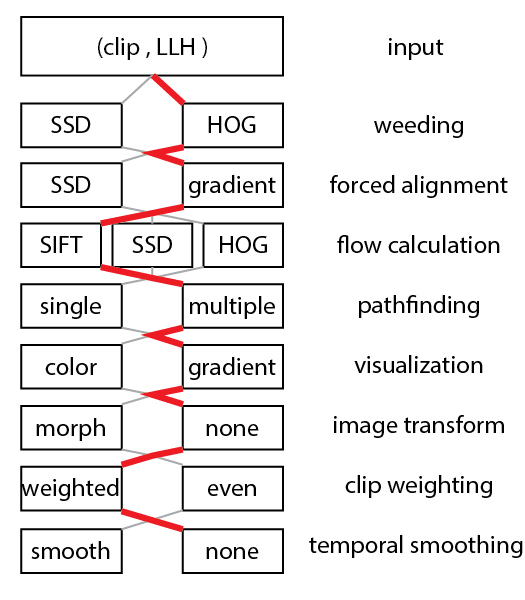
\includegraphics[width=1.0\columnwidth]{figures/system.png}
\caption{We experimented with a variety of options for the five core steps of Preprocessing, Forced Alignment, Flow Calculation, Pathfinding, and Visualization.  Highlighted in red is the most effective path.}
\label{fig:system}
\end{figure}

There are a few processes that we used for several steps in our pipeline, described here for later reference:

\emph{SSD} - Sum of Squared Differences (SSD) is a single number that represents a ``match'' score between two images.  It takes into account differences across the images' respective color channels, squaring and summing those differences to create one number indicating overall different-ness.

\emph{HOG} - Histogram of Oriented Gradients (HOG) descriptors focus on an image's edge data.  The descriptor has a variety of bins representing orientations and locations: images with similar HOG descriptors have similar edge orientations in similar spatial locations.

\emph{Gradient} - An image's gradient represents change in the image rather than absolute values.  Large changes in the image typically correspond to edges.

\subsection{Weeding}
While clips are already "weeded" in some sense by the fMRI data search over the video clip database, in order to make an effective visualization we first discard clips that are obviously very different from each other.  In deference to our already-ranked data, we search for clips that are best aligned to the top-ranked guess at each timestep.

There are two processes for this: \emph{SSD} and \emph{HOG}.  Intuitively, SSD should be better for preserving color in images, since it takes color into account, while HOG should be better at preserving edges in images.  Therefore, we would expect that HOG-weeded guess clips would have better internal edge consistency.  This appears to be true to some degree (see Figure \ref{fig:weeding}): there fore we select HOG as our weeding tool of choice (in spite of SSD's obvious superiority in time efficiency).

\begin{figure}
\centering
    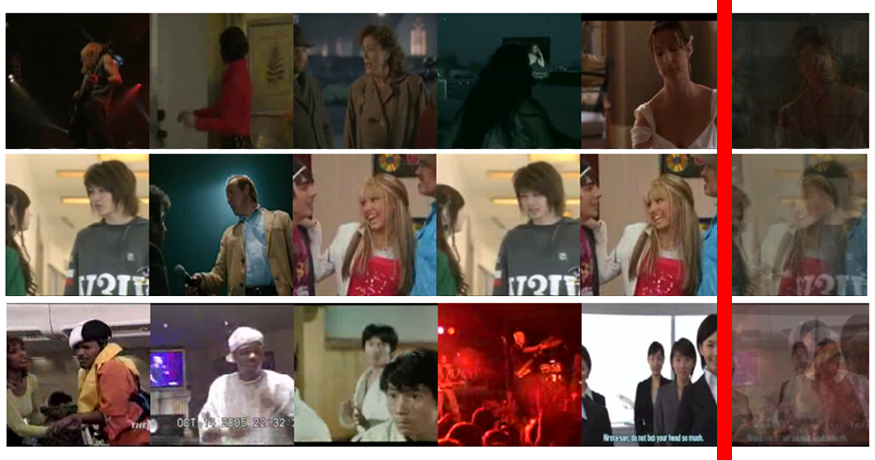
\includegraphics[width=1.0\columnwidth]{figures/preproc.png}
\caption{The top 5 guesses for one frame weeded based on SSD (top), HOG (middle), and LLH (bottom); and the sum of all five images (right).}
\label{fig:weeding}
\end{figure}

\subsection{Forced Alignment}
We forcibly align

\subsection{Flow Calculation}
\valkyrie{write me}

\subsection{Pathfinding}
\natalia{write me}

\subsection{Visualization}
\natalia{write me}

\subsubsection{Gradient Domain}
\natalia{write me}

\subsubsection{Smoothing}
\natalia{write me}

\subsubsection{Overlay}
\natalia{write me}